%%%%%%%%%%%%%%%%%%%%%%%%%%%%%%%%%%%%%%%%%
% Jacobs Landscape Poster
% LaTeX Template
% Version 1.1 (14/06/14)
%
% Created by:
% Computational Physics and Biophysics Group, Jacobs University
% https://teamwork.jacobs-university.de:8443/confluence/display/CoPandBiG/LaTeX+Poster
% 
% Further modified by:
% Nathaniel Johnston (nathaniel@njohnston.ca)
%
% This template has been downloaded from:
% http://www.LaTeXTemplates.com
%
% License:
% CC BY-NC-SA 3.0 (http://creativecommons.org/licenses/by-nc-sa/3.0/)
%
%%%%%%%%%%%%%%%%%%%%%%%%%%%%%%%%%%%%%%%%%

%----------------------------------------------------------------------------------------
%	PACKAGES AND OTHER DOCUMENT CONFIGURATIONS
%----------------------------------------------------------------------------------------

\documentclass[final]{beamer}

\setbeamertemplate{caption}[numbered]{}

\usepackage{pifont} % for dings

% puts R2 in bold in table 3
\makeatletter
\DeclareRobustCommand\bfseries{%
  \not@math@alphabet\bfseries\mathbf
  \fontseries\bfdefault\selectfont
  \boldmath % <-- added
}
\makeatother

\usepackage[scale=1.24]{beamerposter} % Use the beamerposter package for laying out the poster

\usetheme{confposter} % Use the confposter theme supplied with this template

\setbeamercolor{block title}{fg=ngreen,bg=white} % Colors of the block titles
\setbeamercolor{block body}{fg=black,bg=white} % Colors of the body of blocks
\setbeamercolor{block alerted title}{fg=white,bg=dblue!70} % Colors of the highlighted block titles
\setbeamercolor{block alerted body}{fg=black,bg=dblue!10} % Colors of the body of highlighted blocks
% Many more colors are available for use in beamerthemeconfposter.sty

%-----------------------------------------------------------
% Define the column widths and overall poster size
% To set effective sepwid, onecolwid and twocolwid values, first choose how many columns you want and how much separation you want between columns
% In this template, the separation width chosen is 0.024 of the paper width and a 4-column layout
% onecolwid should therefore be (1-(# of columns+1)*sepwid)/# of columns e.g. (1-(4+1)*0.024)/4 = 0.22
% Set twocolwid to be (2*onecolwid)+sepwid = 0.464
% Set threecolwid to be (3*onecolwid)+2*sepwid = 0.708

\newlength{\sepwid}
\newlength{\onecolwid}
\newlength{\twocolwid}
\newlength{\threecolwid}
\setlength{\paperwidth}{48in} % A0 width: 46.8in
\setlength{\paperheight}{36in} % A0 height: 33.1in
\setlength{\sepwid}{0.024\paperwidth} % Separation width (white space) between columns
\setlength{\onecolwid}{0.22\paperwidth} % Width of one column
\setlength{\twocolwid}{0.464\paperwidth} % Width of two columns
\setlength{\threecolwid}{0.708\paperwidth} % Width of three columns
\setlength{\topmargin}{-0.5in} % Reduce the top margin size
%-----------------------------------------------------------

\usepackage{graphicx}  % Required for including images

\usepackage{booktabs} % Top and bottom rules for tables

%----------------------------------------------------------------------------------------
%	TITLE SECTION 
%----------------------------------------------------------------------------------------

\title{Survival Analysis of Questions Posted on the iFixit Answers Forum} % Poster title

\author{Lisa Oshita\footnote{Frost Research Fellow, recipient of the Frost Undergraduate Student Research Award}, Anthony Pileggi, Shannon Pileggi} % Author(s)

\institute{Department of Statistics, California Polytechnic State University} % Institution(s)

%----------------------------------------------------------------------------------------

\begin{document}

\addtobeamertemplate{block end}{}{\vspace*{2ex}} % White space under blocks
\addtobeamertemplate{block alerted end}{}{\vspace*{2ex}} % White space under highlighted (alert) blocks

\setlength{\belowcaptionskip}{2ex} % White space under figures
\setlength\belowdisplayshortskip{2ex} % White space under equations

\begin{frame}[t] % The whole poster is enclosed in one beamer frame

\begin{columns}[t] % The whole poster consists of three major columns, the second of which is split into two columns twice - the [t] option aligns each column's content to the top

\begin{column}{\sepwid}\end{column} % Empty spacer column

\begin{column}{\onecolwid} % The first column

%----------------------------------------------------------------------------------------
%	OBJECTIVES
%----------------------------------------------------------------------------------------

\begin{alertblock}{Overview}

\textcolor{dblue!70}{\ding{228}} iFixit's online question and answer forum, \textit{Answers}, features over 120,000 user-asked questions related specifically to device repair. Analysis of question response times can reveal factors that affect how quickly questions receive answers, which can lead to suggestions for how users can ask better questions to minimize response times and for how forum design can be improved. 

\textcolor{dblue!70}{\ding{228}} \underline{Objective} Develop a Cox proportional hazards model to predict the survival probability (probability that a question remains unanswered beyond a certain time \textit{t}), of questions on the forum, with the goal of identifying variables significantly associated with response time.

\end{alertblock}

%----------------------------------------------------------------------------------------
%	INTRODUCTION
%----------------------------------------------------------------------------------------

\begin{block}{Data}

Data analyzed contained 7,760 questions posted from April 2017 to July 2017. 63.8\% received an answer. Shortest response time was 0.5 hours; longest was 2,159 hours (90 days). Figure 1 shows the distribution of response times for questions analyzed. 

Original variables in the data include: device name and category, question title, text, tags, new user status, post date and answer date. Fourteen variables, capturing textual and user information, were derived from the data.

\end{block}

%------------------------------------------------

\begin{figure}
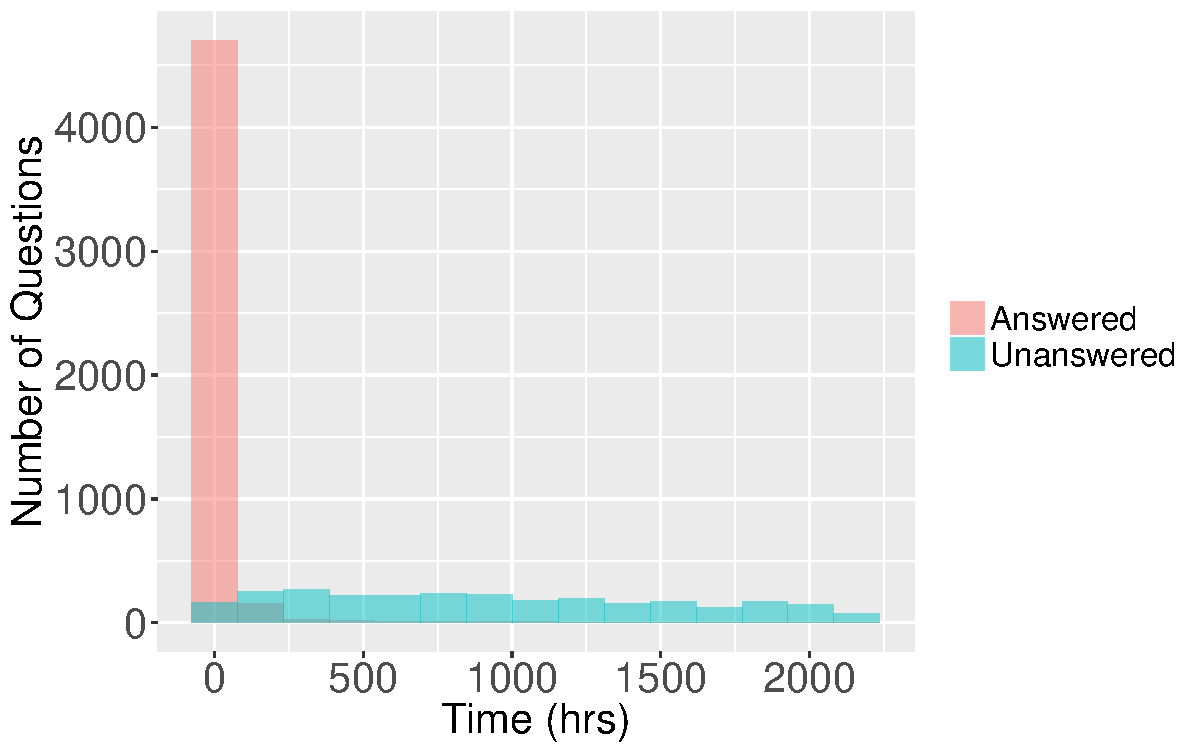
\includegraphics[width=1\linewidth]{FIG1.pdf}
\caption{Distribution of response times}
\label{fig1}
\end{figure}

%----------------------------------------------------------------------------------------

\end{column} % End of the first column

\begin{column}{\sepwid}\end{column} % Empty spacer column

\begin{column}{\twocolwid} % Begin a column which is two columns wide (column 2)

\begin{columns}[t,totalwidth=\twocolwid] % Split up the two columns wide column

\begin{column}{\onecolwid}\vspace{-.6in} % The first column within column 2 (column 2.1)

%----------------------------------------------------------------------------------------
%	METHODS
%----------------------------------------------------------------------------------------

\begin{block}{Methods}

\textcolor{dblue!70}{\ding{228}} \underline{Univariate Analysis} Used to identify which variables, as well as the optimal form of continuous variables (if transformations and restricted cubic splines should be applied), to include in the model.

\textcolor{dblue!70}{\ding{228}} \underline{Five Fold Cross-Validation} In each iteration, the model was built on the training set and used to predict hazard ratios on the test set. 

\textcolor{dblue!70}{\ding{228}} \underline{Assessing Performance} Predicted hazard ratios were entered into separate Cox models as the single quantitative predictor with response times as the survival time. Resulting Nagelkerke's $R^2$ statistic, concordance statistic, Somers' \textit{Dxy}, partial likelihood ratio and p-value, were averaged over each iteration and assessed as performance indicators.  

\textcolor{dblue!70}{\ding{228}} \underline{Final Model} The model was fit to the full data and proportional hazards assumption was assessed.

\end{block}

%----------------------------------------------------------------------------------------
%	MODEL BUILDING RESULTS
%----------------------------------------------------------------------------------------

\begin{block}{Model Building Results}

Univariate analysis determined that all categorical predictors should be retained. Table \ref{table:continuous} shows the form of continuous predictors included in the final model. 

\renewcommand{\arraystretch}{1.2} % to increase the spacing between table rows
\begin{table}[!htbp]
\vspace{2ex}
\begin{tabular}{| l | c |}
    \hline
    \textbf{Predictor} & \textbf{Knots} \\
    \hline
    $\sqrt{\textnormal{average tag frequency}}$ & 0 \\
    $\log\left({\textnormal{average tag length} + 1}\right)$ & 4 \\
    $\sqrt{\textnormal{line breaks / text length}}$ & 5 \\
    $\sqrt{\textnormal{line breaks / text length}}$ & 3 \\
    $\log\left({\textnormal{text length}}\right)$ & 5 \\
    \hline
\end{tabular}
\caption{Form of continuous predictors included in the final model (knots indicates the number of knots included in restricted cubic splines}
\label{table:continuous}
\end{table}

Table \ref{table:1} displays the average performance metrics for models fit to test and training sets in cross-validation, as well as metrics for the model fit to the full data. Results for training, test, and the full data did not change significantly, indicating that the model was not over fit. 

\end{block}


%----------------------------------------------------------------------------------------

\end{column} % End of column 2.1

\begin{column}{\onecolwid}\vspace{-.6in} % The second column within column 2 (column 2.2)

%----------------------------------------------------------------------------------------
%	FINAL MODEL RESULTS
%----------------------------------------------------------------------------------------

\begin{block}{Final Model Results}

\underline{Final model statistics} 

\textcolor{dblue!70}{\ding{228}} PLR $=$ 1265.29 (p-value \textless0.0001)

\textcolor{dblue!70}{\ding{228}} $R^2 =$ 0.15

\textcolor{dblue!70}{\ding{228}} Somers' \textit{Dxy} $=$ 0.27 

\underline{Significant Predictors} Device category, if the question was posted on a weekend or a weekday, whether or not the question's title contained at least one word considered frequently-used among unanswered questions, whether or not the question's title ends in a question mark.

\begin{table}[!htbp]
\vspace{3ex}
\begin{tabular}{|r|r|r|r|r|r|r|r|} % FIX THE R2 HERE 
  \hline
  & \textbf{HR} & \textbf{LR} & \textbf{p-value} & \textbf{$R^2$} & \textbf{\textit{Dxy}} & \textbf{C} \\ 
  \hline
  \textbf{Training} & 2.03 & 937.39  & \textless0.0001 & 0.14 & 0.27 & 0.63 \\ 
  \textbf{Test}     & 1.99 & 220.83  & \textless0.0001 & 0.14 & 0.26 & 0.63 \\
  \textbf{Full}     & 2.03 & 1165.03 & \textless0.0001 & 0.14 & 0.28 & 0.63 \\ 
  \hline
\end{tabular}
\caption{Performance metrics (HR: Hazard Ratio, LR: Partial Likelihood Ratio, C: Concordance)} 
\label{table:1}
\end{table}

Assessing the proportional hazards assumption indicated that several levels of the device categorization variable violated the assumption. 

\end{block}

%----------------------------------------------------------------------------------------
%	INTERPRETING HAZARD
%----------------------------------------------------------------------------------------

\begin{block}{Interpreting Hazard}

Hazard is approximately equivalent to the conditional probability that a question will receive an answer within the next moment in time, given that it has not already received an answer. Table \ref{table:hr} contains interpretations of select hazard coefficients of the final model.

\end{block}

%----------------------------------------------------------------------------------------
%	SUGGESTIONS
%----------------------------------------------------------------------------------------

\begin{block}{Suggestions}

Results from this analysis lead to suggestions for changes in CQA design. Many users incorrectly specified device names and tags (e.g. a user asking a question about a Turtle Beach Ear Force XO ONE headset defined the device name as, ``Turtle Beach Ear Force Xmy grandson chewed through the wire while he was playing it's brand-new is there anyway I can have it fixed0 One'').

\end{block}

%----------------------------------------------------------------------------------------

\end{column} % End of column 2.2

\end{columns} % End of the split of column 2 - any content after this will now take up 2 columns width

\begin{columns}[t,totalwidth=\twocolwid] % Split up the two columns wide column again

\begin{column}{\onecolwid} % The first column within column 2 (column 2.1)
%----------------------------------------------------------------------------------------

\end{column} % End of column 2.1

\begin{column}{\onecolwid} % The second column within column 2 (column 2.2)

\end{column} % End of column 2.2

\end{columns} % End of the split of column 2

\end{column} % End of the second column

\begin{column}{\sepwid}\end{column} % Empty spacer column

\begin{column}{\onecolwid} % The third column

%----------------------------------------------------------------------------------------
%	HAZARD INTERPRETATIONS + SUGGESTIONS 
%----------------------------------------------------------------------------------------

\begin{block}

\renewcommand{\arraystretch}{1.15} % to increase the spacing between table rows
\begin{table}[!htbp]
\begin{tabular}{|p{26cm}|} 
  \hline
  The estimated hazard of receiving an answer is 154\% higher (95\% CI (132\%, 179\%)) for questions pertaining to Apple products than the hazard for questions about Android and Other phones, controlling for all other predictors. \\ \hline
  The estimated hazard of receiving an answer is 25\% lower (95\% CI (19\%, 29\%)) for questions with titles that contain at least one word considered to be frequently-used among unanswered questions, than the hazard for questions with titles that do not, controlling for all other predictors. \\ \hline
  The estimated hazard of receiving an answer for questions posted on a weekend is 13\% lower (95\% CI (7\%, 18\%)) than the hazard for questions posted on a weekday, controlling for all other predictors. \\ \hline
  \hline
\end{tabular}
\caption{Hazard coefficient interpretations} 
\label{table:hr}
\end{table}

It is likely that these inconsistencies contributed to the final model's low predictive power. This, along with the results of the final model, reveal some ways the CQA can be structured to potentially decrease response times. As findings indicate that questions with correctly defined tags and device names may lead to quicker response times, the CQA can provide a stricter framework for asking questions by restricting tags or devices users can include to a drop-down list. The CQA can also include more tips to guide users asking questions. Implementing a more structured framework for asking questions can help users create understandable and clear questions and in turn decrease response time, as well as create a set of consistent questions for improved analysis. 

\end{block}

%----------------------------------------------------------------------------------------
%	ACKNOWLEDGEMENTS
%----------------------------------------------------------------------------------------

\setbeamercolor{block title}{fg=red,bg=white} % Change the block title color

\begin{block}{Acknowledgements}

\small{\rmfamily{This research was supported by the Bill and Linda Frost fund of the California Polytechnic State University of San Luis Obispo. We also thank iFixit for providing access to the CQA data.}} \\

\end{block}


%----------------------------------------------------------------------------------------
%	CONTACT INFORMATION
%----------------------------------------------------------------------------------------

% \setbeamercolor{block alerted title}{fg=black,bg=norange} % Change the alert block title colors
% \setbeamercolor{block alerted body}{fg=black,bg=white} % Change the alert block body colors
% 
% \begin{alertblock}{Contact Information}
% 
% \begin{itemize}
% \item Web: \href{http://www.university.edu/smithlab}{http://www.university.edu/smithlab}
% \item Email: \href{mailto:john@smith.com}{john@smith.com}
% \item Phone: +1 (000) 111 1111
% \end{itemize}
% 
% \end{alertblock}
% 
% \begin{center}
% \begin{tabular}{ccc}
% \includegraphics[width=0.4\linewidth]{logo.png} & \hfill & \includegraphics[width=0.4\linewidth]{logo.png}
% \end{tabular}
% \end{center}

%----------------------------------------------------------------------------------------

\end{column} % End of the third column

\end{columns} % End of all the columns in the poster

\end{frame} % End of the enclosing frame

\end{document}
